\section{Finite models and a controllable contact geometry}
\label{sec:finite}

We first reduce a signed spin Hamiltonian to a half-filled Hubbard model.
The geometric construction is part of this reduction: every Hubbard
hopping will later be set by a small displacement of a nuclear site.
For a finite-dimensional self-adjoint operator $A$, write $E(A)$ for its
smallest eigenvalue.  On two spin-$1/2$ sites set
\[
 h^s_{ij}=X_iX_j+Y_iY_j+Z_iZ_j
          =\boldsymbol\sigma_i\cdot\boldsymbol\sigma_j.
\]
Its eigenvalues are $-3$ on the singlet and $1$ on the triplet, so
$\lVert h^s_{ij}\rVert=3$.

\Needspace{14\baselineskip}
\subsection{The source problem and a quantitative perturbation bound}

\begin{theorem}[Source problem]\label{thm:source}
There is a QMA-complete promise problem whose Hamiltonians are
\[
 H_{\rm in}=\sum_{e=LR}J_e h^s_{LR}
\]
on finite, nonwrapping subgraphs of the square lattice, with no
one-qubit terms.  The signed weights $J_e$ are rational.  The number of
vertices and edges, the lattice extent, the weight magnitudes, and the
threshold magnitudes are bounded by fixed polynomials in the source
size $n\geq2$.  The rational thresholds $a_s<b_s$ have separation
$\delta_s=b_s-a_s\geq1/\poly(n)$.
\end{theorem}

This is the square-lattice Heisenberg consequence of
\cite[Theorem~48 and Section~10.1]{CMP2019}, using the polynomial-weight
spatially sparse branch of Lemma~47 there. The Heisenberg interaction has
rank-three coupling matrix, so it is outside the exceptional rank-one
family in that theorem; the square-lattice construction has no one-qubit
fields. The following normalization makes the encoding interface explicit.

Let $\delta>0$ be a known rational inverse-polynomial lower bound on the
incoming gap, let $q_s$ be the number of weighted edges, and put
$\varepsilon_0=\delta/100$. Round each edge coefficient within
$\varepsilon_0/\max\{1,q_s\}$. Since $\|h^s_{ij}\|=3$, the resulting
Hamiltonian changes by norm at most $3\varepsilon_0$. If the source also
has an identity coefficient $c_0$ and thresholds $a_0,b_0$, approximate
each of those three numbers within $\varepsilon_0$, obtaining
$\widetilde c_0,\widetilde a_0,\widetilde b_0$. For the rounded Hamiltonian
with its identity term removed, set
\[
 a_s=\widetilde a_0-\widetilde c_0+5\varepsilon_0,
 \qquad
 b_s=\widetilde b_0-\widetilde c_0-5\varepsilon_0.
\]
The two threshold approximation errors and the Hamiltonian error sum to
at most $5\varepsilon_0$, so both promises survive. Moreover,
$b_s-a_s\ge\delta-12\varepsilon_0>0$. All rational descriptions have
polynomial length. A connected grid component with $v$ vertices has
coordinate diameter at most $v-1$, by following its lattice paths;
translating components into disjoint strips gives polynomial extent.
These are normalization steps applied to the cited source, not additional
conclusions imported from its statement.

This imported source theorem is the only hardness theorem we need.
In what follows zero-weight edges are omitted. No lower bound
on the magnitudes of the remaining weights is assumed, and no total-spin
sector is selected.
By appending an isolated original vertex if necessary, at a lattice
position outside the existing finite drawing, we may assume that there
is at least one original vertex.  Tensoring with its uncoupled spin
preserves the minimum energy and all polynomial bounds.

We use the following finite-dimensional estimate twice.  It controls the
bottom energy and does not require a gap within the encoded subspace.
The effective second-order operator is the familiar one from
Schrieffer--Wolff perturbation theory; see
Bravyi, DiVincenzo, and Loss~\cite[Section~3.2]{BravyiDiVincenzoLoss2011}.
We prove the particular bound needed here directly, so its constants and
the empty-complement case are explicit.

\begin{lemma}[Second-order bottom-energy estimate]
\label{lem:second-order}
Let $A\geq0$ be a finite-dimensional self-adjoint operator, let
$P\neq0$ project onto its kernel, and put $Q=I-P$.  Suppose
$A\geq gQ$ for some $g>0$.  Let $B=B^*$ satisfy $PBP=0$ and
$\lVert B\rVert\leq\epsilon g$, where $0\leq\epsilon<1/2$.
Define $A^{-1}$ to vanish on $P$.  Then
\begin{equation}\label{eq:second-order-bound}
 \left|E(A+B)-E\bigl(-PBA^{-1}BP\big|_{P}\bigr)\right|
 \leq 2g\epsilon^3.
\end{equation}
The conclusion also holds when $Q=0$.
\end{lemma}

\begin{proof}
Let $K=PBA^{-1}BP\geq0$ and $\kappa=\lVert K\rVert$.
Since $Bp\in Q$ for $p\in P$,
\begin{equation}\label{eq:second-order-size}
 0\leq\kappa\leq\frac{\lVert B\rVert^2}{g}
                  \leq g\epsilon^2.
\end{equation}
For $p\in P$ and $q\in Q$, the inequality
$QBQ\geq-\epsilon gQ\geq-\epsilon A|_Q$ gives
\begin{align*}
 \langle p+q,(A+B)(p+q)\rangle
 &\geq (1-\epsilon)\langle q,Aq\rangle
       +2\operatorname{Re}\langle q,Bp\rangle\\
 &= (1-\epsilon)
    \left\|A^{1/2}q+\frac{A^{-1/2}Bp}{1-\epsilon}\right\|^2
       -\frac{\langle p,Kp\rangle}{1-\epsilon}.
\end{align*}
On a unit vector this is at least $-\kappa/(1-\epsilon)$.
Consequently
\[
 E(A+B)+\kappa
 \geq-\frac{\epsilon\kappa}{1-\epsilon}
 \geq-2g\epsilon^3.
\]

For the other direction choose a unit $p\in P$ with $Kp=\kappa p$
and set $q=-A^{-1}Bp$.  Then $\lVert q\rVert\leq\epsilon$ and
\[
 \langle p+q,(A+B)(p+q)\rangle
       =-\kappa+\langle q,Bq\rangle.
\]
Writing $r=\lVert q\rVert^2$, the variational principle therefore gives
\[
 E(A+B)+\kappa
 \leq \frac{\langle q,Bq\rangle+\kappa r}{1+r}
 \leq g\epsilon^3+g\epsilon^4
 \leq\tfrac32g\epsilon^3.
\]
The smallest eigenvalue of $-K$ on $P$ is $-\kappa$, proving the
claim.  If $Q=0$, the hypothesis $PBP=0$ forces $B=0$, and the same
formulas hold with all inverse terms zero.
\end{proof}

\subsection{Replacing signed bonds by positive Heisenberg bonds}

Piddock and Montanaro's singlet mediator construction changes the sign of
an effective interaction by coupling to the same or to opposite members
of a strongly bound pair~\cite[Section~2.4 and Lemma~5]{PiddockMontanaro2017}.
We use its isotropic specialization below, keeping the scalar shift and
the simultaneous-gadget error explicit. This stage produces only positive
spin bonds; the next geometric stage assigns each of them a controllable
unit contact.

For every source edge $e=LR$ introduce two ancillary spins $A_e,B_e$.
There are $k$ such pairs.  Define
\begin{equation}\label{eq:positive-gadget}
 \begin{split}
 v_e&=\sqrt{2|J_e|},\qquad
 C_e=\begin{cases}A_e,&J_e<0,\\ B_e,&J_e>0,\end{cases}\\
 H_+&=\Delta\sum_e h^s_{A_eB_e}
    +\sqrt\Delta\sum_e v_e
          \bigl(h^s_{LA_e}+h^s_{RC_e}\bigr).
 \end{split}
\end{equation}
Every nonzero coefficient in $H_+$ is positive.  Put
\begin{equation}\label{eq:spin-shift}
 V=\sum_e v_e,\qquad
 C_0=3k\Delta+\frac32\sum_e v_e^2.
\end{equation}

\begin{proposition}[Positive-spin reduction]\label{prop:positive-spin}
If $\sqrt\Delta>3V$, then
\begin{equation}\label{eq:positive-spin-error}
 \bigl|E(H_+)-E(H_{\rm in})+C_0\bigr|
       \leq\frac{27V^3}{\sqrt\Delta}.
\end{equation}
In particular, a polynomially large integer $\Delta$ makes this error
an arbitrarily small prescribed inverse polynomial.
\end{proposition}

\begin{proof}
Take
\[
 A=\Delta\sum_e(h^s_{A_eB_e}+3I),\qquad
 B=\sqrt\Delta\sum_e v_e(h^s_{LA_e}+h^s_{RC_e}).
\]
The kernel of $A$ consists of arbitrary original spins tensored with a
singlet on each ancillary pair.  Denote its projection by $P_s$.
The gap is $g=4\Delta$, and
\[
 P_sBP_s=0,\qquad
 \lVert B\rVert\leq6\sqrt\Delta V.
\]
A weak interaction from pair $e$ takes that pair's singlet into its
triplet space and leaves every other ancillary pair in its singlet.
Thus every state reached from $P_s$ in one hop has excitation energy
$4\Delta$.  Moreover, terms associated with distinct pairs give zero
mixed second-order contributions: a term acting on pair $f\neq e$
cannot remove the triplet on pair $e$.  This remains true when the two
source edges share an original vertex.

For a singlet $|s\rangle$ on $A,B$ and Pauli components $\mu,\nu$,
\[
 \langle s|\sigma_A^\mu\sigma_A^\nu|s\rangle
       =\delta_{\mu\nu},\qquad
 \langle s|\sigma_A^\mu\sigma_B^\nu|s\rangle
       =-\delta_{\mu\nu}.
\]
Consequently the squares of the two weak terms each compress to $3I$.
Their two ordered cross terms sum to $2h^s_{LR}$ when $C_e=A_e$,
and to $-2h^s_{LR}$ when $C_e=B_e$.  The contribution of pair $e$ to
$-P_sBA^{-1}BP_s$, identified with an operator on the original spins,
is therefore
\begin{equation}\label{eq:spin-gadget-effective}
 -\frac{v_e^2}{4}
 \begin{cases}
  6I+2h^s_{LR},&J_e<0,\\
  6I-2h^s_{LR},&J_e>0
 \end{cases}
 =J_e h^s_{LR}-\frac32v_e^2 I.
\end{equation}
The factor $4$ in the denominator is the singlet--triplet excitation
energy in units of $\Delta$.

Apply Lemma~\ref{lem:second-order} with
$\epsilon=3V/(2\sqrt\Delta)<1/2$.  Its error bound is
$2(4\Delta)\epsilon^3=27V^3/\sqrt\Delta$.
Since $A+B=H_++3k\Delta I$, summing
\eqref{eq:spin-gadget-effective} gives the result.  If $k=0$, both
perturbation and shift vanish and the assertion is exact.
\end{proof}

Here is one explicit scale choice, which we retain for later bookkeeping.
Set
\begin{equation}\label{eq:spin-scale}
 \begin{split}
 \gamma&=\min\{1,\delta_s\},\qquad
 W=\max\bigl(\{1\}\cup\{|J_e|:e\}\bigr),\\
 \overline V&=\max\{1,2kW\},\qquad
 \Delta=\left\lceil
       \left(\frac{1728\overline V^3}{\gamma}\right)^2
             \right\rceil.
 \end{split}
\end{equation}
Then $V\leq\overline V$, and
\eqref{eq:positive-spin-error} is at most $\gamma/64$.
Furthermore $v_e\leq\sqrt\Delta$, so every coefficient of $H_+$ is
at most $\Delta$.  All these scales have polynomial magnitude in $n$.
Intermediate square roots cause no encoding issue: their nonnegative
values admit polynomial-precision rational approximations by bisection.

\subsection{Contact geometry and independent length control}

Place the original lattice vertices at spacing $2$ in the $x,y$ plane.
Orient each source edge in the positive $x$ or positive $y$ direction.
Use local coordinates $(\ell,\zeta)$, where $\ell$ is distance from its
left endpoint along that direction, and $\zeta=z$ for a horizontal edge
but $\zeta=-z$ for a vertical edge.  The two ancillas are placed at
\begin{equation}\label{eq:gadget-coordinates}
 \begin{array}{c|cc}
       & A_e & B_e\\ \hline
 J_e<0 &(1,0)&(1,1)\\[2pt]
 J_e>0 &(1/2,\sqrt3/2)&(3/2,\sqrt3/2).
 \end{array}
\end{equation}
The local endpoints are always $L=(0,0)$ and $R=(2,0)$.
Let $p_1,\ldots,p_m$ denote all original and ancillary sites.
Their coordinates belong to $\mathbb Q(\sqrt3)^3$ and have polynomial
bit descriptions.
\Cref{fig:gadgets} shows these placements and the additional contact
between consecutive positive gadgets.

\begin{figure}[tbp]
\centering
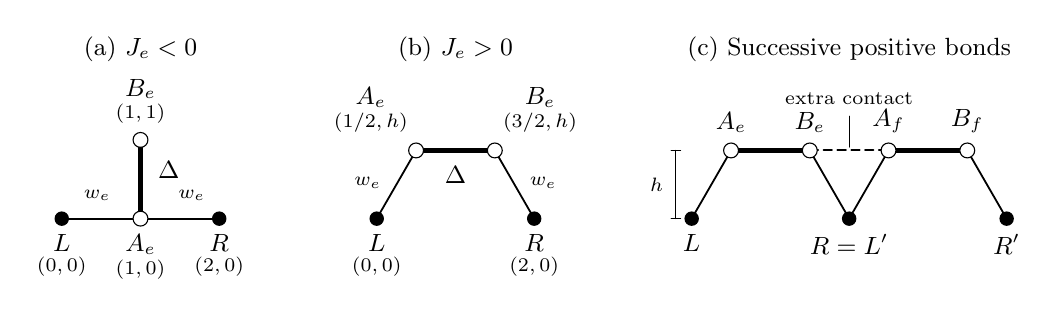
\begin{tikzpicture}[
 x=1cm,y=1cm,line cap=round,
 original/.style={circle,fill=black,draw=black,inner sep=1.7pt},
 ancilla/.style={circle,fill=white,draw=black,inner sep=1.9pt},
 weak/.style={line width=0.65pt},
 strong/.style={line width=1.5pt},
 extra/.style={densely dashed,line width=0.75pt},
 every node/.style={font=\small}]
 \begin{scope}
  \node at (1,2.15) {(a) $J_e<0$};
  \draw[weak] (0,0)--(1,0)--(2,0);
  \draw[strong] (1,0)--(1,1);
  \node[original] at (0,0) {};
  \node[original] at (2,0) {};
  \node[ancilla] at (1,0) {};
  \node[ancilla] at (1,1) {};
  \node[anchor=north] at (0,-0.08)
       {\shortstack{$L$\\[-1pt]\scriptsize$(0,0)$}};
  \node[anchor=north] at (1,-0.08)
       {\shortstack{$A_e$\\[-1pt]\scriptsize$(1,0)$}};
  \node[anchor=north] at (2,-0.08)
       {\shortstack{$R$\\[-1pt]\scriptsize$(2,0)$}};
  \node[anchor=south] at (1,1.08)
       {\shortstack{$B_e$\\[-1pt]\scriptsize$(1,1)$}};
  \node[anchor=west] at (1.10,0.62) {$\Delta$};
  \node[font=\scriptsize,anchor=south] at (0.45,0.10) {$w_e$};
  \node[font=\scriptsize,anchor=south] at (1.65,0.10) {$w_e$};
 \end{scope}
 \begin{scope}[shift={(4,0)}]
  \node at (1,2.15) {(b) $J_e>0$};
  \draw[weak] (0,0)--(0.5,0.8660254);
  \draw[weak] (1.5,0.8660254)--(2,0);
  \draw[strong] (0.5,0.8660254)--(1.5,0.8660254);
  \node[original] at (0,0) {};
  \node[original] at (2,0) {};
  \node[ancilla] at (0.5,0.8660254) {};
  \node[ancilla] at (1.5,0.8660254) {};
  \node[anchor=north] at (0,-0.08)
       {\shortstack{$L$\\[-1pt]\scriptsize$(0,0)$}};
  \node[anchor=north] at (2,-0.08)
       {\shortstack{$R$\\[-1pt]\scriptsize$(2,0)$}};
  \node[anchor=south east] at (0.52,0.97)
       {\shortstack{$A_e$\\[-1pt]\scriptsize$(1/2,h)$}};
  \node[anchor=south west] at (1.48,0.97)
       {\shortstack{$B_e$\\[-1pt]\scriptsize$(3/2,h)$}};
  \node[anchor=north] at (1,0.79) {$\Delta$};
  \node[font=\scriptsize,anchor=east] at (0.18,0.45) {$w_e$};
  \node[font=\scriptsize,anchor=west] at (1.82,0.45) {$w_e$};
 \end{scope}
 \begin{scope}[shift={(8,0)}]
  \node at (2,2.15) {(c) Successive positive bonds};
  \draw[weak] (0,0)--(0.5,0.8660254);
  \draw[weak] (1.5,0.8660254)--(2,0)--(2.5,0.8660254);
  \draw[weak] (3.5,0.8660254)--(4,0);
  \draw[strong] (0.5,0.8660254)--(1.5,0.8660254);
  \draw[strong] (2.5,0.8660254)--(3.5,0.8660254);
  \draw[extra] (1.5,0.8660254)--(2.5,0.8660254);
  \foreach \x in {0,2,4} {\node[original] at (\x,0) {};}
  \foreach \x in {0.5,1.5,2.5,3.5}
       {\node[ancilla] at (\x,0.8660254) {};}
  \node[anchor=north] at (0,-0.08) {$L$};
  \node[anchor=north] at (2,-0.08) {$R=L'$};
  \node[anchor=north] at (4,-0.08) {$R'$};
  \node[anchor=south] at (0.5,0.97) {$A_e$};
  \node[anchor=south] at (1.5,0.97) {$B_e$};
  \node[anchor=south] at (2.5,0.97) {$A_f$};
  \node[anchor=south] at (3.5,0.97) {$B_f$};
  \draw[thin] (-0.2,0)--(-0.2,0.8660254);
  \draw[thin] (-0.26,0)--(-0.14,0);
  \draw[thin] (-0.26,0.8660254)--(-0.14,0.8660254);
  \node[anchor=east,font=\scriptsize] at (-0.24,0.433) {$h$};
  \draw[thin] (2,1.30)--(2,0.91);
  \node[font=\scriptsize,anchor=south] at (2,1.32)
       {extra contact};
 \end{scope}
\end{tikzpicture}
\caption{The contact construction in the local $(\ell,\zeta)$ plane,
with $h=\sqrt3/2$ and $w_e=\sqrt\Delta\,v_e$.
Filled vertices are original spins and open vertices are ancillas.
Every solid segment has length one; thick segments carry weight
$\Delta$ and thin segments the indicated weak weight.  The dashed
segment in (c) is an additional unit contact, with weight zero in
$H_+$; it receives only the small positive hopping floor in the Hubbard
model.  Horizontal gadgets use $\zeta=z$, and vertical gadgets use
$\zeta=-z$.}
\label{fig:gadgets}
\end{figure}

\begin{lemma}[Contact classification]\label{lem:contact-layout}
All the sites $p_i$ are distinct.  Every pair is either at distance one
or at distance at least $\sqrt2$.  The complete set $\mathcal C$ of
unit-distance pairs consists of:
\begin{enumerate}
 \item $L A_e$, $A_e R$, and $A_e B_e$ for a negative source edge;
 \item $L A_e$, $A_e B_e$, and $B_e R$ for a positive source edge;
 \item $B_e A_f$ for two consecutive positive source edges $e,f$ on
       the same original lattice line.
\end{enumerate}
Thus every interaction of $H_+$ is a contact.  Its weight on a contact
will be denoted $K_{ij}\geq0$, using $K_{ij}=0$ for contacts in the
third class.
\end{lemma}

\begin{proof}
Within one gadget the assertion follows directly from
\eqref{eq:gadget-coordinates}.  For a negative gadget the two distances
from $B_e$ to original endpoints are $\sqrt2$; for a positive gadget
the two nonadjacent endpoint--ancilla distances are $\sqrt3$.
Original vertices are mutually separated by at least $2$.
An original vertex other than the endpoints of an ancilla's gadget,
on that same axis line, has along-line distance at least $3/2$ to a
positive ancilla and at least $3$ to a negative midpoint.
An original vertex off that line differs in a transverse coordinate
by at least $2$.

For ancillas belonging to distinct gadgets on the same axis line,
the only along-line separation below $3/2$ is the separation $1$
between $B_e$ and $A_f$ for consecutive positive gadgets.  They have
the same height and hence are a contact.  All remaining such pairs
are at least $3/2>\sqrt2$ apart.  Distinct parallel axis lines have
transverse separation at least $2$.

It remains to compare horizontal and vertical ancillas.  Call an
ancilla \emph{midpoint type} if it belongs to a negative gadget,
and \emph{positive type} otherwise.  Two midpoint-type projections
differ by at least $1$ in each planar coordinate, so their distance
is at least $\sqrt2$.  A midpoint-type and a positive-type projection
differ by at least $1$ and $1/2$ in the two planar coordinates.
Their heights differ by at least $\sqrt3/2$, since horizontal and
vertical heights have opposite signs.  Their squared distance is
therefore at least $1+1/4+3/4=2$.  Finally two positive-type ancillas
from perpendicular directions have height difference $\sqrt3$,
already larger than $\sqrt2$.  These cases exhaust all pairs and
also establish distinctness.
\end{proof}

Orient each contact arbitrarily and write
$u_{ij}=p_j-p_i$, so $|u_{ij}|=1$.  Its first-order length change under
site displacements $s_i$ is $u_{ij}\cdot(s_j-s_i)$.  Reversing the
orientation reverses both factors and leaves this scalar unchanged.
The following stronger-than-counting fact is what permits independent
hopping calibration.

\begin{lemma}[A bounded right inverse for contact lengths]
\label{lem:displacement}
For every real assignment $(d_{ij})_{\{i,j\}\in\mathcal C}$ there
are displacements $s_i\in\mathbb R^3$ such that
\begin{equation}\label{eq:contact-displacement}
 u_{ij}\cdot(s_j-s_i)=d_{ij},\qquad
 \max_i|s_i|\leq6m\max_{\mathcal C}|d_{ij}|.
\end{equation}
For an empty contact set take all displacements zero.  The construction
is linear in $d$, uses polynomially many arithmetic operations with
coefficients in $\mathbb Q(\sqrt3)$, and has no consistency condition
around lattice cycles.
\end{lemma}

\begin{proof}
Set the height displacement of every original vertex to zero.
The horizontal coordinate of each original vertex will be determined
using only its original row, and its vertical planar coordinate using
only its original column.  These are independent variables even when
both directions meet at the same vertex.

Fix one such axis line.  Write $a$ for displacement along it, $z$
for physical height displacement, and put $\sigma=1$ for a horizontal
line and $\sigma=-1$ for a vertical line.  On every connected run of
negative bonds choose the first original $a$ coordinate to be zero,
and accumulate
\begin{equation}\label{eq:negative-displacement}
 \begin{split}
 a_R&=a_L+d_{LA_e}+d_{A_eR},\qquad
 a_{A_e}=a_L+d_{LA_e},\\
 a_{B_e}&=a_{A_e},\qquad
 z_{A_e}=0,\qquad z_{B_e}=\sigma d_{A_eB_e}.
 \end{split}
\end{equation}
Unconstrained original coordinates may be set to zero.  A positive
or missing bond places no requirement on the difference of its
original endpoints' $a$ coordinates at this step, so it separates
runs.  Each run is a path on a line, and
\eqref{eq:negative-displacement} satisfies all three constraints in
its negative gadgets.

Now consider the elevated vertices of positive gadgets on this line.
Their same-height contacts, including the extra contacts of
Lemma~\ref{lem:contact-layout}, form disjoint paths.  Set the first
$a$ coordinate on each path to zero and successively set
$a_{\rm next}=a_{\rm current}+d_{\rm edge}$.
Every such contact vector is along the axis, so its constraint
involves only these $a$ coordinates.  Each elevated vertex has
exactly one additional, sloped contact to an original vertex.
Writing $h_0=\sqrt3/2$, set
\begin{equation}\label{eq:positive-displacement}
 \begin{split}
 z_{A_e}&=\frac{d_{LA_e}-(a_{A_e}-a_L)/2}{\sigma h_0},\\
 z_{B_e}&=\frac{d_{B_eR}-(a_R-a_{B_e})/2}{\sigma h_0}.
 \end{split}
\end{equation}
Indeed the two unit spoke vectors are
$\tfrac12 e_{\rm axis}+\sigma h_0 e_z$ and
$\tfrac12 e_{\rm axis}-\sigma h_0 e_z$, respectively.
Because the original height displacements vanish, these formulas
satisfy the remaining equations without imposing any new condition
on original coordinates.  Set each ancilla's unused transverse
coordinate to zero.

Repeat on all rows and columns.  The row procedure changes only
original $x$ coordinates, and the column procedure only original
$y$ coordinates.  No ancilla belongs to both procedures.  Thus the
constructions do not overwrite each other.  In particular a square
cycle is not a cycle in either scalar accumulation graph; its vector
closure is automatic because actual vertex displacements have been
assigned.

For the norm bound put $d_{\max}=\max_{\mathcal C}|d_{ij}|$.
Every original along-line coordinate has magnitude at most
$2m d_{\max}$, and every accumulated elevated coordinate has
magnitude at most $m d_{\max}$.  Negative ancilla coordinates
have magnitude at most $(2m+1)d_{\max}$ along the line and at
most $d_{\max}$ in height.  From
\eqref{eq:positive-displacement}, positive ancilla heights are at
most $(1+3m/2)d_{\max}/h_0$.  Combining at most two nonzero
coordinates at any site gives the stated bound $6m d_{\max}$.
All assignments are additions and multiplication by fixed rational
numbers or by $1/h_0$, proving the algorithmic assertion.
\end{proof}

Only approximate length equations will be needed.  To make their bit
complexity explicit, suppose the data are known within $\tau/4$ and
apply the displayed right inverse to those approximations.  Approximate
its output and $Dp_i$, then round to rational positions $X_i$, with
total Euclidean error at most $\tau/4$ per site.  Defining
$s_i=X_i-Dp_i$ absorbs this rounding even though the $p_i$ may be
irrational.  Every contact equation then has error at most
$\tau/4+2(\tau/4)<\tau$, and
\begin{equation}\label{eq:rounded-displacement}
 \max_i|s_i|\leq6m\bigl(\max_{\mathcal C}|d_{ij}|+\tau\bigr)+\tau.
\end{equation}
The number of arithmetic operations is polynomial, and all accumulated
coefficients have polynomial size.  Computing $\sqrt3$ and the other
real inputs to sufficiently many additional polynomially bounded bits
therefore gives the stated absolute accuracy in polynomial time.
In particular this does not call for an ill-conditioned general
linear-system solve.

For later use, actual distances satisfy the exact vector identities
and the elementary estimates
\begin{equation}\label{eq:displaced-geometric-bounds}
 \begin{aligned}
 X_j-X_i&=D u_{ij}+s_j-s_i
                       &&(\{i,j\}\in\mathcal C),\\
 |X_j-X_i|&=D+u_{ij}\cdot(s_j-s_i)+O(S^2/D)
                       &&(\{i,j\}\in\mathcal C),\\
 |X_j-X_i|&\geq\sqrt2D-2S
                       &&(\{i,j\}\notin\mathcal C),
 \end{aligned}
\end{equation}
provided $\max_i|s_i|\leq S$ and $S\leq D/4$.  The middle estimate
is the Taylor bound for the Euclidean norm away from zero.  The last
is the triangle inequality and Lemma~\ref{lem:contact-layout}.
No exact nonlinear prescribed-length problem is being solved; the
quadratic remainder will be included in the hopping estimates.

\subsection{The half-filled Hubbard model}

We now realize those positive bonds as second-order hopping processes.
Virtual double occupancy gives the antiferromagnetic superexchange
mechanism of Anderson~\cite{Anderson1959}. In our Pauli-matrix
normalization the coefficient is $t^2/U$ multiplying
$h^s_{ij}-I$. We calculate the fermionic signs below and retain the
constant term, because it contributes to the final decision thresholds.

Associate two fermionic modes, labelled $\uparrow,\downarrow$, to each
of the $m$ sites and restrict to exactly $m$ fermions.  Let
$c_{i\sigma}^\dagger,c_{i\sigma}$ satisfy the canonical
anticommutation relations and put
$n_{i\sigma}=c_{i\sigma}^\dagger c_{i\sigma}$.
For nonnegative hopping strengths define
\begin{equation}\label{eq:hubbard-definition}
 \begin{split}
 H_{\rm Hub}(t)
   &=-\sum_{\{i,j\}\in\mathcal C}\sum_{\sigma=\uparrow,\downarrow}
       t_{ij}\bigl(c_{i\sigma}^\dagger c_{j\sigma}
                  +c_{j\sigma}^\dagger c_{i\sigma}\bigr)
       +U\sum_i n_{i\uparrow}n_{i\downarrow},\\
 U&=\iint_{\mathbb R^3\times\mathbb R^3}
       \frac{\phi(y)^2\phi(y')^2}{|y-y'|}\,\dd y\,\dd y',
       \qquad \phi(y)=\pi^{-1/2}e^{-|y|}.
 \end{split}
\end{equation}
The radial probability density of $\phi^2$ is $p(r)=4r^2e^{-2r}$.
Angular integration gives the kernel $1/\max(r,s)$: for $r,s>0$,
\[
 \frac12\int_{-1}^{1}\frac{\dd u}{\sqrt{r^2+s^2-2rsu}}
      =\frac1{\max(r,s)}.
\]
Since $\int_0^r p(s)\,\dd s=1-e^{-2r}(1+2r+2r^2)$,
\begin{equation}\label{eq:onsite-integral}
 \begin{split}
 U&=8\int_0^\infty r e^{-2r}
           \bigl[1-e^{-2r}(1+2r+2r^2)\bigr]\,\dd r\\
  &=8\left(\frac14-\frac1{16}-\frac1{16}-\frac3{64}\right)
    =\frac58.
 \end{split}
\end{equation}
Thus $U$ is a fixed positive rational constant.

Let $q_{\mathcal C}=|\mathcal C|$ and define the rational scales
\begin{equation}\label{eq:hubbard-scales}
 \overline R=\max\{1,q_{\mathcal C}\Delta\},\qquad
 \eta=\frac{U\gamma}{1024\overline R^3},\qquad
 \alpha=\frac{\eta^2}{U},\qquad
 f=\frac{\alpha\gamma}{128\max\{1,q_{\mathcal C}\}}.
\end{equation}
The ideal hoppings are $t^{(0)}_{ij}=\eta\sqrt{K_{ij}}$.
For each contact compute a rational $r_{ij}$ with
$|r_{ij}-t^{(0)}_{ij}|\leq f$, and output
\begin{equation}\label{eq:hopping-floor}
 t_{ij}=\max\{f,r_{ij}\}.
\end{equation}
Polynomial-precision bisection on nonnegative square roots (at most
two nested square roots here) suffices to compute $r_{ij}$; no exact
comparison between irrational numbers is required.  The maximum in
\eqref{eq:hopping-floor} is a comparison of rationals.  All final
hoppings satisfy $1/\poly(n)\leq t_{ij}<1$, including those with
$K_{ij}=0$.

\begin{proposition}[Hubbard reduction with rational hoppings]
\label{prop:hubbard}
The construction above is deterministic and polynomial time.  With
\begin{equation}\label{eq:finite-scalar-shift}
 C_s=C_0+\sum_{\{i,j\}\in\mathcal C}K_{ij}
     =3k\Delta+\frac32\sum_e v_e^2
                        +\sum_{\{i,j\}\in\mathcal C}K_{ij},
\end{equation}
it satisfies
\begin{equation}\label{eq:finite-combined-error}
 \left|E\bigl(H_{\rm Hub}(t)\bigr)
            -\alpha\bigl(E(H_{\rm in})-C_s\bigr)\right|
        \leq\frac{3\alpha\gamma}{64}.
\end{equation}
The scalar $C_s$ has polynomial magnitude and can be approximated to
any polynomial-bit absolute precision in polynomial time.
\end{proposition}

\begin{proof}
First use the ideal hoppings $t^{(0)}$.  Let
$A_U=U\sum_i n_{i\uparrow}n_{i\downarrow}$ and let $T$ be the hopping
part of $H_{\rm Hub}(t^{(0)})$.  At filling $m$, the kernel of $A_U$
is exactly the singly occupied subspace: having $m$ fermions, at most
one at each of $m$ sites, forces precisely one per site.  Identify this
subspace with $m$ spins, and denote its projection by $P_{\rm so}$.
The complementary excitation energies are positive integer multiples
of $U$.  A single hop from $P_{\rm so}$ creates one vacant site
and one doubly occupied site and hence has energy exactly $U$.
In particular $P_{\rm so}TP_{\rm so}=0$.

A second hop can return to single occupancy only by moving an electron
from that doubly occupied site to that vacant site.  Thus the two hops
must use the same unordered bond; products from different bonds have
zero compression, even when the bonds share a vertex.
For completeness, consider one bond $i,j$ of strength $t$, with local
mode order $i\uparrow,i\downarrow,j\uparrow,j\downarrow$.
Write $|D_i\rangle=c_{i\uparrow}^\dagger
c_{i\downarrow}^\dagger|0\rangle$ and similarly for $|D_j\rangle$.
The bond hopping operator $T_{ij}$ obeys
\[
 T_{ij}|\uparrow,\downarrow\rangle
      =-t(|D_i\rangle+|D_j\rangle),\qquad
 T_{ij}|\downarrow,\uparrow\rangle
      = t(|D_i\rangle+|D_j\rangle).
\]
It consequently annihilates all triplets and maps the singlet to
$-\sqrt2t(|D_i\rangle+|D_j\rangle)$, of squared norm $4t^2$.
In an ordering containing other sites between $i$ and $j$, those sites
are singly occupied during this two-hop process; their fixed fermion
parity changes transition phases but not the compressed product.
Equivalently, permuting the intervening mode pairs gives the same
calculation under a fermionic change of basis.  It follows that
\begin{equation}\label{eq:hubbard-exchange}
 -P_{\rm so}T_{ij}A_U^{-1}T_{ij}P_{\rm so}
       =-\frac{4t^2}{U}P_{{\rm singlet},ij}
       =\frac{t^2}{U}(h^s_{ij}-I).
\end{equation}
Here $P_{{\rm singlet},ij}=(I-h^s_{ij})/4$.

For each spin, $c_{i\sigma}^\dagger c_{j\sigma}
+c_{j\sigma}^\dagger c_{i\sigma}$ has norm one, so
\[
 \lVert T\rVert\leq2\sum_{\mathcal C}t^{(0)}_{ij}
       =2\eta\sum_{\mathcal C}\sqrt{K_{ij}}
       \leq2\eta\overline R.
\]
The last inequality uses $K_{ij}\leq\Delta$ and $\Delta\geq1$.
Lemma~\ref{lem:second-order}, with $g=U$ and
$\epsilon=2\eta\overline R/U<1/2$, and
\eqref{eq:hubbard-exchange} give
\begin{equation}\label{eq:ideal-hubbard-error}
 \left|E\bigl(H_{\rm Hub}(t^{(0)})\bigr)
       -\alpha\left(E(H_+)-\sum_{\mathcal C}K_{ij}\right)\right|
 \leq\frac{16\eta^3\overline R^3}{U^2}
 \leq\frac{\alpha\gamma}{64}.
\end{equation}
If the complementary subspace is empty, as can happen for $m=1$,
there is no hopping and this assertion is exact.

For the rational hoppings, nonnegativity of $t^{(0)}_{ij}$ and the
accuracy of $r_{ij}$ imply
$|\max\{f,r_{ij}\}-t^{(0)}_{ij}|\leq f$.
Therefore
\begin{equation}\label{eq:hopping-rounding-error}
 \left\|H_{\rm Hub}(t)-H_{\rm Hub}(t^{(0)})\right\|
      \leq2q_{\mathcal C}f\leq\frac{\alpha\gamma}{64}.
\end{equation}
Also $t^{(0)}_{ij}\leq\eta\overline R\leq U/1024$ and
$f\leq U/(128\cdot1024^2)$, which verify $f\leq t_{ij}<1$.
The floor $f$ is an inverse polynomial.  This argument covers an ideal
hopping much smaller than $f$ and an ideal hopping equal to zero; no
coefficient lower bound has been used.  If $\mathcal C$ is empty,
\eqref{eq:hopping-rounding-error} is simply zero.

Finally, Proposition~\ref{prop:positive-spin} with
\eqref{eq:spin-scale} contributes at most another
$\alpha\gamma/64$.  Adding the three errors proves
\eqref{eq:finite-combined-error}.  All sizes, magnitudes, and reciprocal
precision budgets in the construction are polynomial in $n$.
Each $K_{ij}$ is either $\Delta$, a square root of the rational number
$2\Delta|J_e|$, or zero.  The displayed scalar shift is thus efficiently
approximable to the asserted precision, completing the proof.
\end{proof}
